% !TEX program = pdflatex
\documentclass[aspectratio=169,11pt]{beamer}
% Shared Beamer layout. Compile from the individual talk directory.
\usepackage[T1]{fontenc}
\usepackage[ngerman]{babel}
\usepackage{tgheros}

\definecolor{StreetshotsInk}{HTML}{17232B}
\definecolor{StreetshotsMuted}{HTML}{485861}
\definecolor{StreetshotsLink}{HTML}{15596D}
\definecolor{StreetshotsRule}{HTML}{DCE2E5}

\setbeamercolor{background canvas}{bg=white}
\setbeamercolor{normal text}{fg=StreetshotsInk,bg=white}
\setbeamercolor{structure}{fg=StreetshotsInk}
\setbeamercolor{subtitle}{fg=StreetshotsMuted}
\setbeamercolor{caption}{fg=StreetshotsMuted}
\setbeamercolor{footline}{fg=StreetshotsInk,bg=white}
\setbeamerfont{frametitle}{size=\Large,series=\bfseries}
\setbeamerfont{title}{size=\huge,series=\bfseries}
\setbeamerfont{subtitle}{size=\large}
\setbeamerfont{footline}{size=\scriptsize,series=\bfseries}

\setbeamersize{text margin left=9mm,text margin right=9mm}
\setbeamertemplate{navigation symbols}{}
\setbeamertemplate{itemize item}{\raisebox{0.26ex}{\rule{0.43ex}{0.43ex}}}
\setbeamertemplate{itemize subitem}{\raisebox{0.25ex}{\rule{0.65ex}{0.12ex}}}
\addtobeamertemplate{itemize/enumerate body begin}{}{\setlength{\itemsep}{0.52em}}
\addtobeamertemplate{itemize/enumerate subbody begin}{}{\setlength{\itemsep}{0.30em}}

\setbeamertemplate{frametitle}{%
  \nointerlineskip
  \begin{beamercolorbox}[wd=\paperwidth,leftskip=9mm,rightskip=9mm]{frametitle}
    \vskip4.4mm%
    \usebeamerfont{frametitle}\insertframetitle\par
    \vskip1.5mm%
  \end{beamercolorbox}%
}

\setbeamertemplate{footline}{%
  \begin{beamercolorbox}[wd=\paperwidth]{footline}
    {\color{StreetshotsRule}\hrule height 0.25pt}%
    \vskip1.6mm%
    \hbox to \paperwidth{%
      \hskip9mm%
      \raisebox{1.45mm}{\usebeamerfont{footline}\href{https://streetshots.io/}{streetshots.io}}%
      \hfil
      
\includegraphics[height=5.4mm]{../../assets/HS_PF_logo_20170502.jpg}%
      \hskip9mm%
    }%
    \vskip1.7mm%
  \end{beamercolorbox}%
}

\graphicspath{{../../assets/}}

\title{Verkehrszeichenkataster}
\subtitle{streetshots.io für Pforzheim}
\author{Prof. Dr. Raphael Volz}
\date{20. November 2026}

\newcommand{\websource}[2]{\href{#1}{\textcolor{StreetshotsLink}{#2}}}
\newcommand{\screenshotframe}[2]{%
  \begin{frame}{#1}
    \centering
    \includegraphics[width=\linewidth,height=62mm,keepaspectratio]{#2}
  \end{frame}%
}

\begin{document}

\begin{frame}
  \begin{columns}[c,onlytextwidth]
    \begin{column}{0.70\textwidth}
      {\usebeamerfont{title}\inserttitle\par}
      \vspace{2.0mm}
      {\usebeamerfont{subtitle}\usebeamercolor[fg]{subtitle}\insertsubtitle\par}
      \vspace{8mm}
      {\insertauthor\par}
      \vspace{1.1mm}
      {\small\color{StreetshotsMuted}\insertdate\par}
    \end{column}
    \begin{column}{0.25\textwidth}
      \centering
      
\includegraphics[width=\linewidth]{Pforzheim-768x806.png}
    \end{column}
  \end{columns}
\end{frame}

\begin{frame}{Wer bin ich?}
  \begin{itemize}
    \item Seit 2012 Professor für Angewandte Informatik an der Hochschule Pforzheim (Fakultät für Technik)
    \item Seit 2024 Studiengangleiter Intelligente Mobilität 
    (Spezialisierung Wirtschaftsing.)
    \item Sabbatical (50\,\% im Wintersemester 2026/27 und Sommersemester 2027) zur Überarbeitung der Lehre: Entwicklung von youspeed.de als Basis für Computer Vision
    \item Seit 2015 Verkehrszeichenerkennung als Thema im Fach Künstliche Intelligenz (Master)
    \item 2008 Gründung der Moonshots Studios GmbH
    \item 2003 Promotion in KI mit Auszeichnung am KIT
    \item Seit 1993 kommerzielle Softwareentwicklung
    \item nogago (2009--2012), Offline-Navigation für Wandern und Radfahren auf BlackBerry
  \end{itemize}
\end{frame}

\begin{frame}{Was ist youspeed.de}
  \begin{columns}[c,onlytextwidth]
    \begin{column}{0.45\textwidth}
      \begin{itemize}
        \item Advanced Driver Assistance für jedes Auto
        \item Anzeige gültiger Verkehrszeichen
        \item Dashcam
        \item Straßenfotos
        \item Fahrtenbuch
        \item \textbf{USP} Bußgeldberechnung ad hoc
      \end{itemize}
    \end{column}
    \begin{column}{0.52\textwidth}
      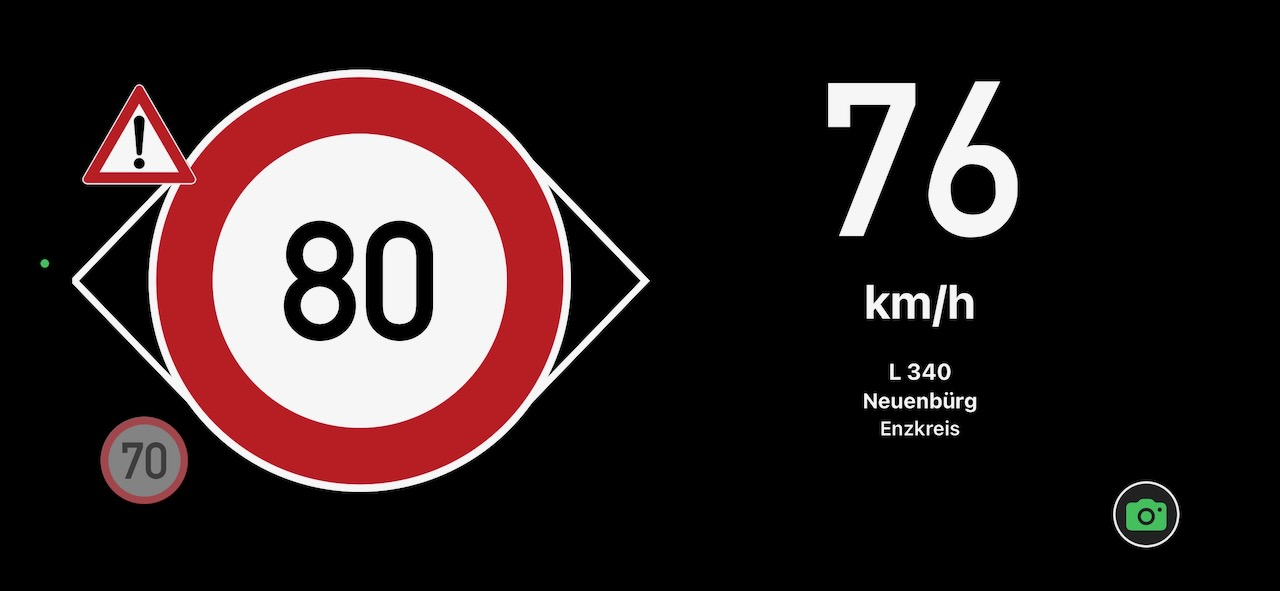
\includegraphics[width=\linewidth]{v15-youspeed-iphone-all-landscape.jpeg}
    \end{column}
  \end{columns}
\end{frame}

\begin{frame}{Was ist streetshots.io}
  \begin{columns}[c,onlytextwidth]
    \begin{column}{0.48\textwidth}
      \begin{itemize}
        \item Kommerzielle Produktidee für Kommunen, Kreise und Länder
        \item \textbf{USP} Gemeinsame Plattform für Kommunen und Bürger
        \item Erster Dienst: Verkehrszeichenkataster
        \item Weitere Dienste für Open Street Intelligence geplant
        \item Beispiel: Straßenschäden erkennen
        \item Später: Baumkataster, Müllerkennung und mehr
      \end{itemize}
    \end{column}
    \begin{column}{0.49\textwidth}
      \centering
      \href{https://www.streetshots.io/}{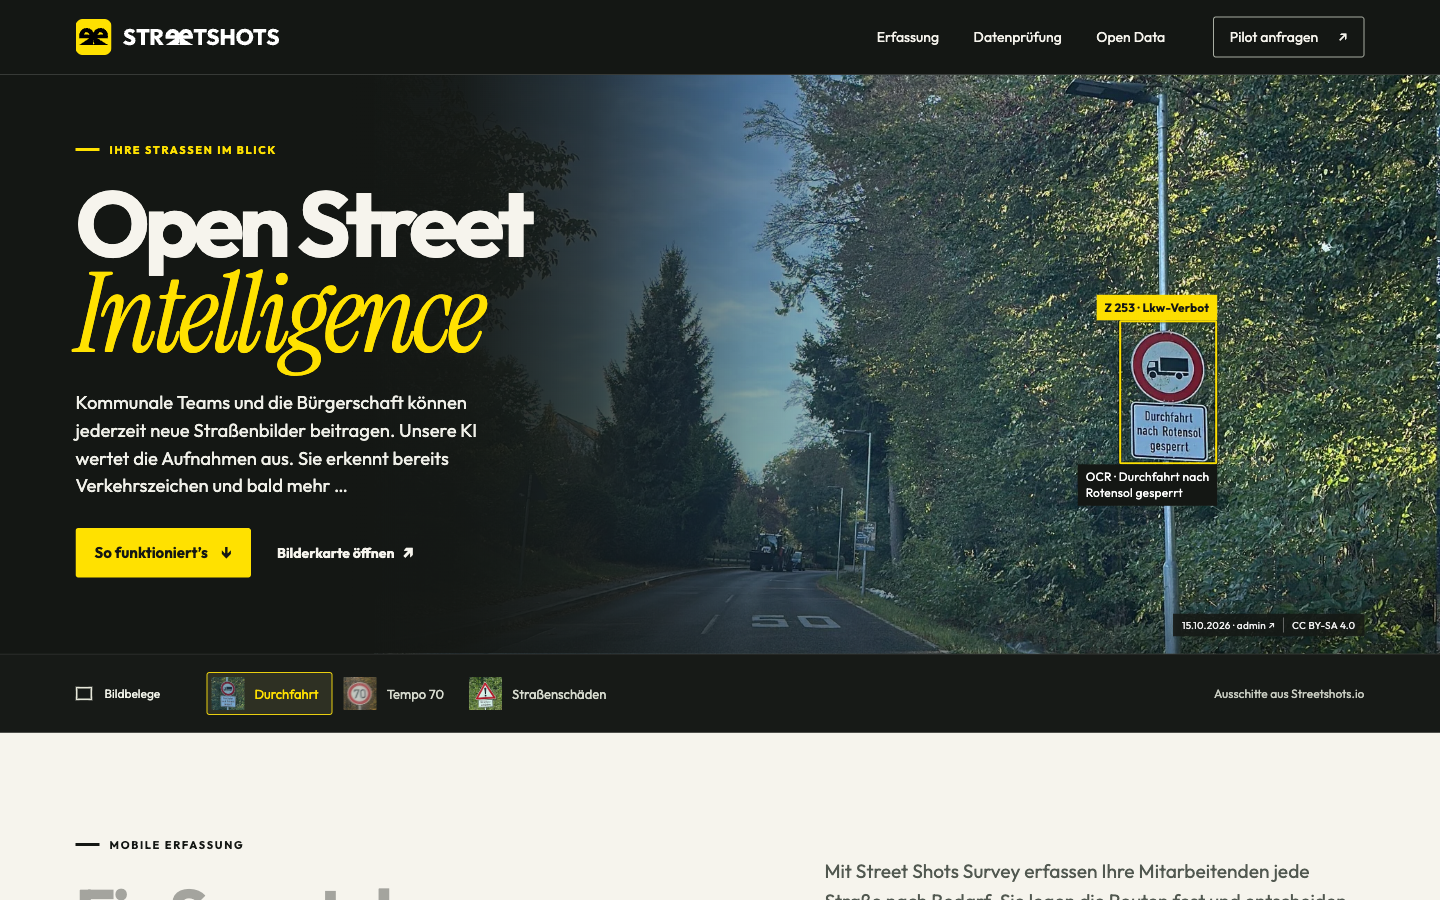
\includegraphics[width=\linewidth]{streetshots-website.png}}\par
      \vspace{1.8mm}
      {\small\websource{https://www.streetshots.io/}{www.streetshots.io}\par}
    \end{column}
  \end{columns}
\end{frame}

% Vector export of assets/architecture.odg.
\screenshotframe{Architektur}{architecture.pdf}

\begin{frame}{Streetshots Survey}
  \begin{columns}[c,onlytextwidth]
    \begin{column}{0.36\textwidth}
      \begin{itemize}
        \item Profi-App für Kommunen
        \item Straßenbilder jederzeit erfassen
        \item Ergänzung oder Ersatz für eine einmalige Befahrung
        \item Erfasste Daten exportieren oder in Streetshots hochladen
      \end{itemize}
    \end{column}
    \begin{column}{0.61\textwidth}
      \centering
      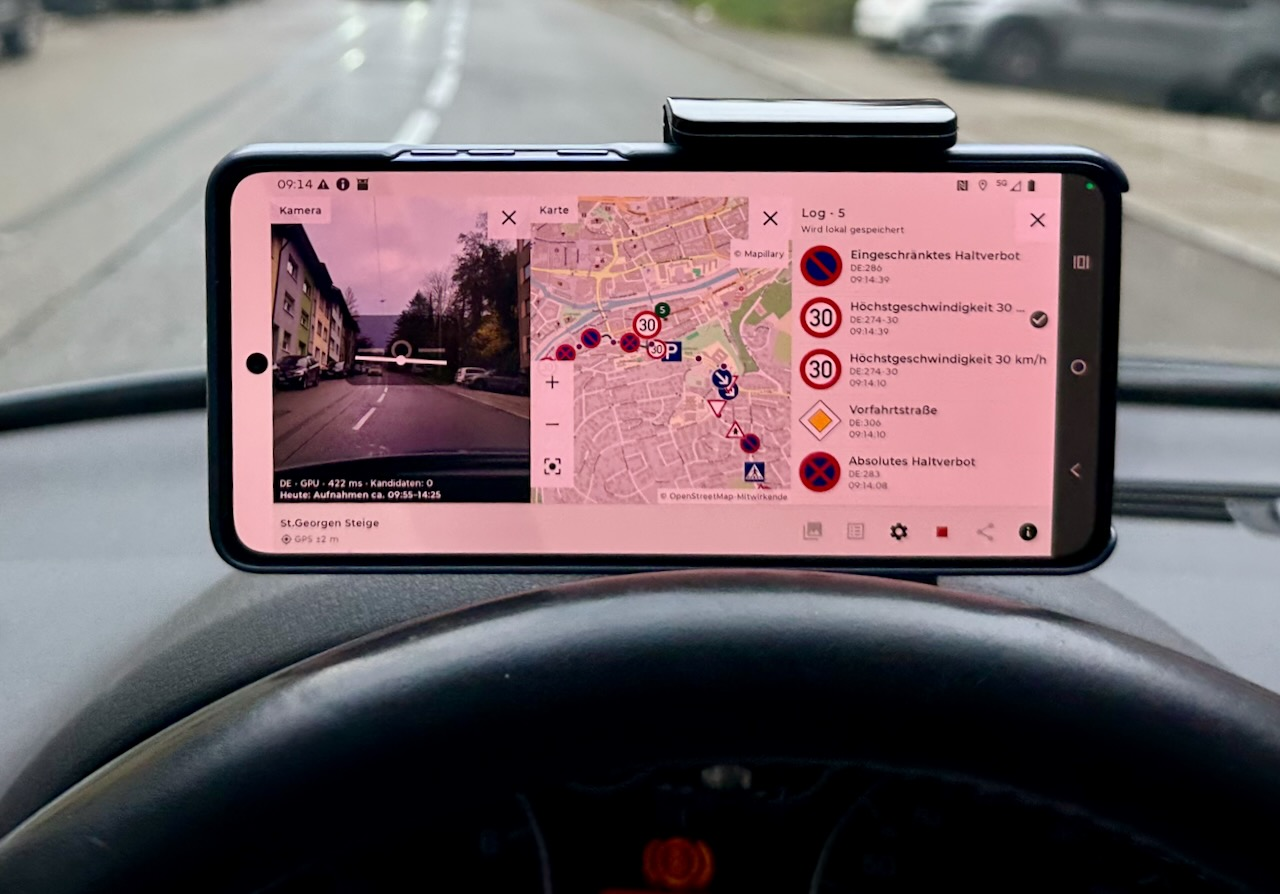
\includegraphics[width=\linewidth,height=56mm,keepaspectratio]{v01-survey-android-all-incar-zoomed.jpeg}\par
      \vspace{1.8mm}
      {\small\usebeamercolor[fg]{caption}Streetshots Survey im Einsatz\par}
    \end{column}
  \end{columns}
\end{frame}

\newcommand{\streetviewurl}{https://images.streetshots.io/?focus=pic&map=17/48.845817/8.444542&pic=019f583b-d864-48f6-8e22-e269ad61a71c&seq=738736dc-4efb-4070-92e8-e0bfd350c63f&speed=250&theme=default&users=default&xyz=170.00/0.00/30}

\begin{frame}{images.streetshots.io}
  \begin{columns}[c,onlytextwidth]
    \begin{column}{0.36\textwidth}
      \begin{itemize}
        \item Open-Source-Straßenansichten
        \item Basis: Panoramax
        \item Darstellung erkannter Objekte
        \item Bearbeitung und Benutzerkonten
        \item Bildsequenzen
        \item Eigene Erweiterung: OCR
      \end{itemize}
    \end{column}
    \begin{column}{0.61\textwidth}
      \centering
      \href{\streetviewurl}{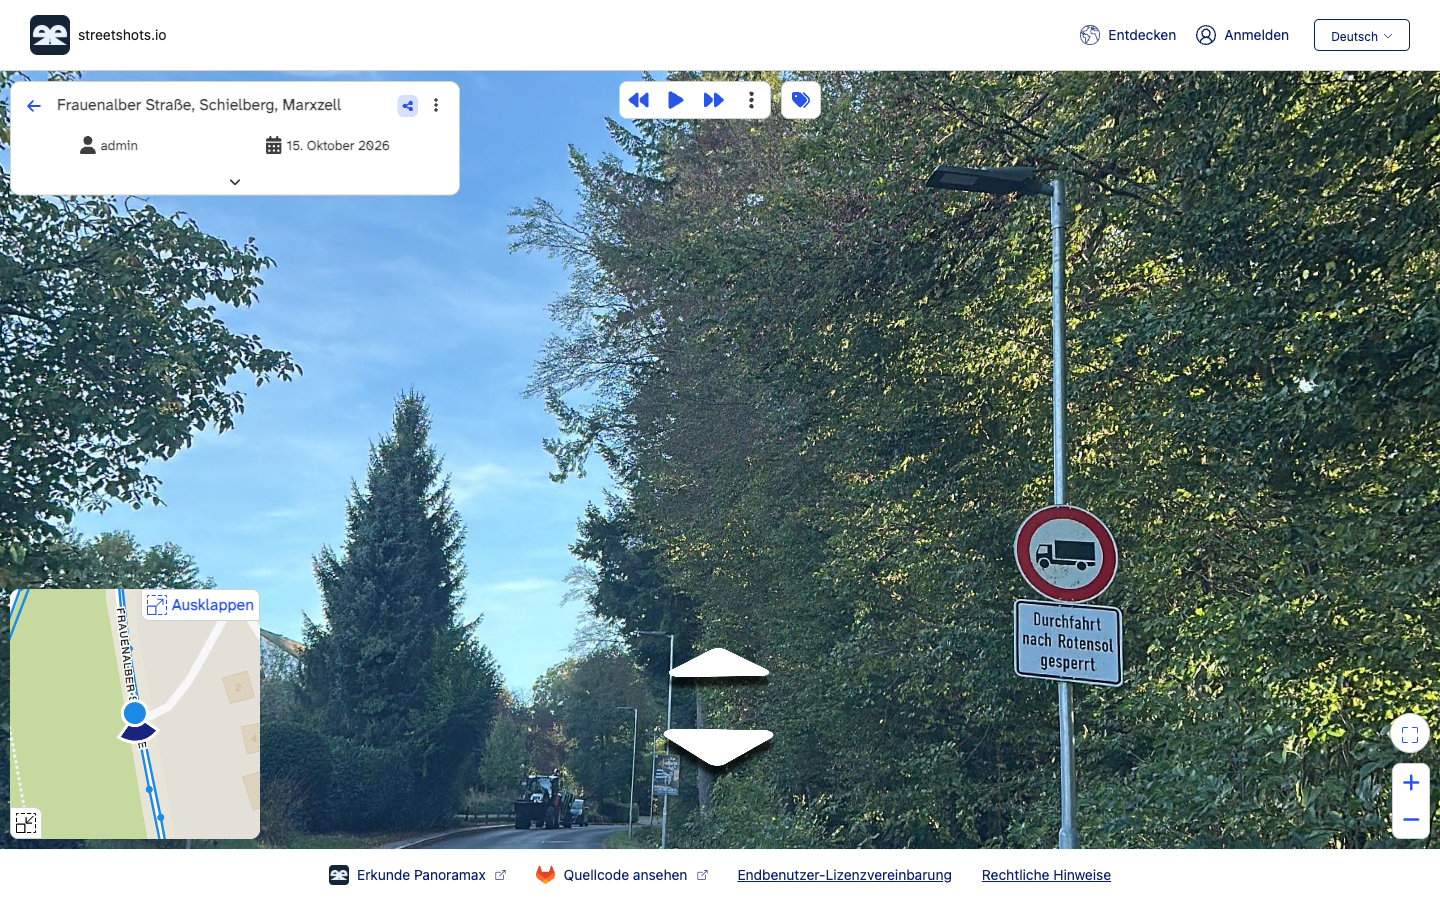
\includegraphics[width=\linewidth]{streetshots-images.png}}\par
      \vspace{1.8mm}
      {\small\websource{\streetviewurl}{images.streetshots.io}\par}
    \end{column}
  \end{columns}
\end{frame}

\begin{frame}{inspector.streetshots.io}
  \begin{columns}[c,onlytextwidth]
    \begin{column}{0.36\textwidth}
      \begin{itemize}
        \item Verkehrszeichenkataster
        \item Aufgezeichnete Befahrungen
        \item Kartenebenen mit weiteren Open-Data-Angeboten
        \item Eigenes Kataster pflegen
        \item Analyseumgebung
        \item Training zur Verbesserung der KI
      \end{itemize}
    \end{column}
    \begin{column}{0.61\textwidth}
      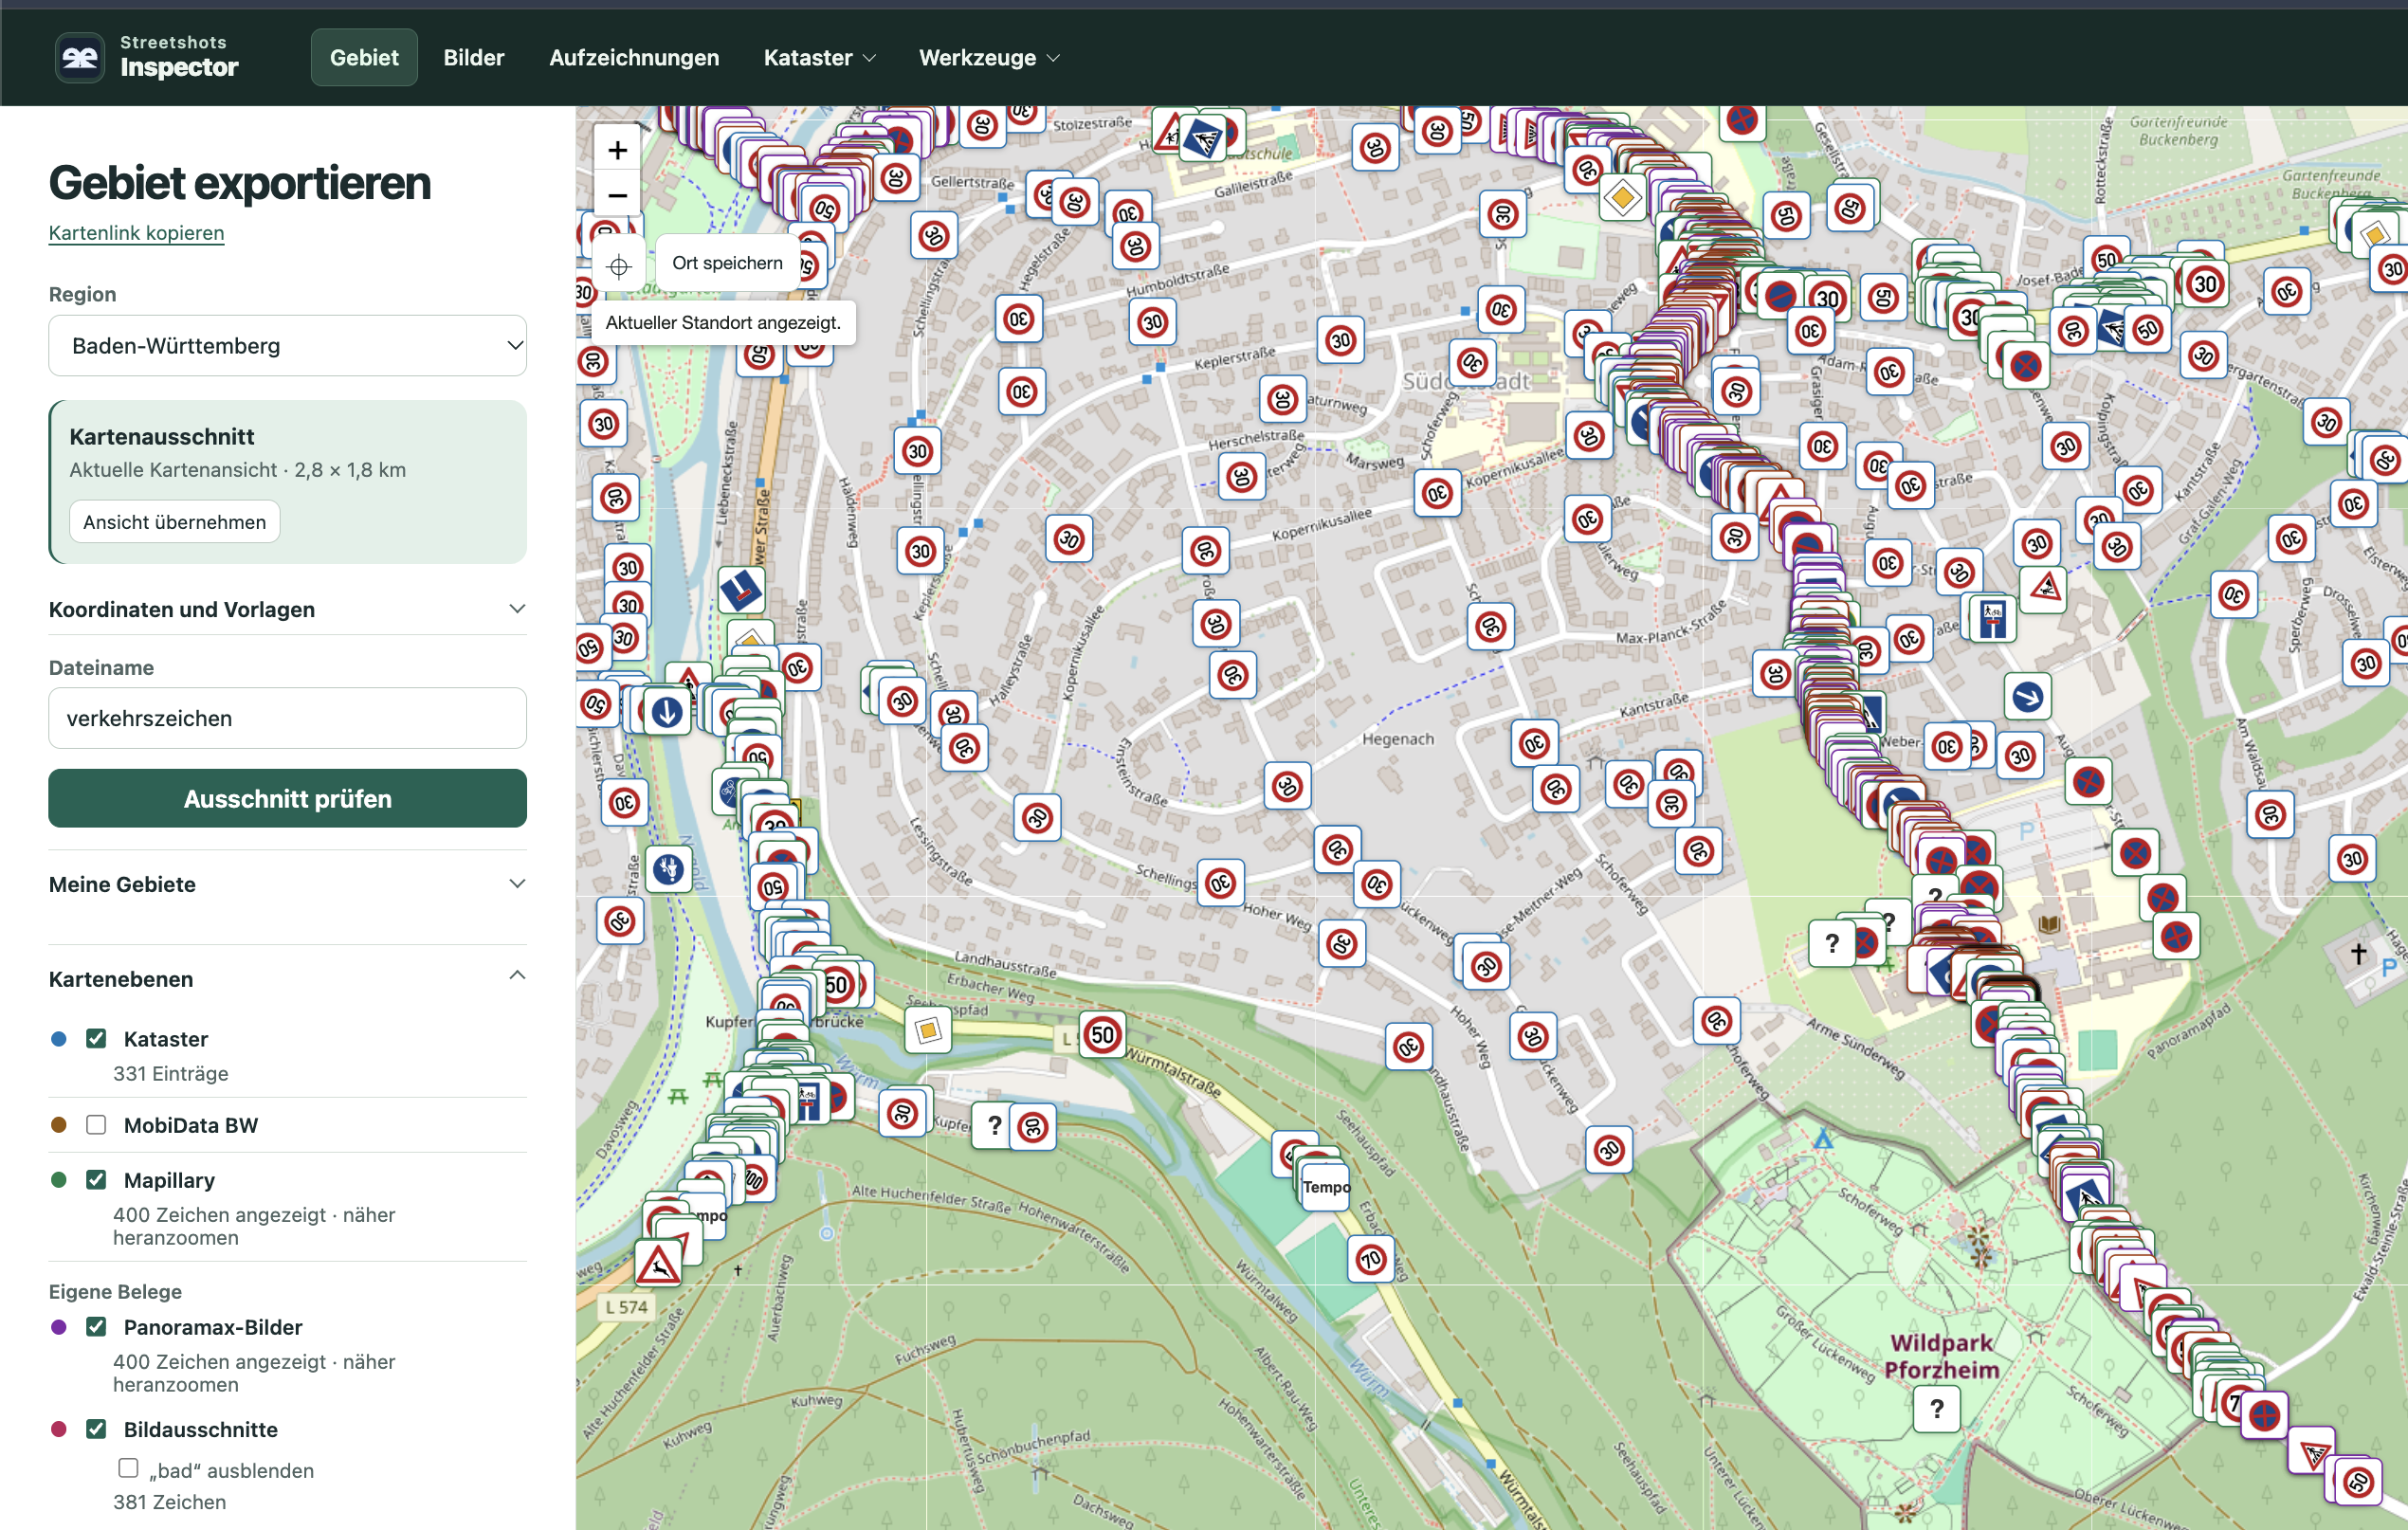
\includegraphics[width=\linewidth]{inspector.Gebiet-Ebenen.png}
    \end{column}
  \end{columns}
\end{frame}

\begin{frame}{Streetshots.io KI Modelle}
  \begin{itemize}
    \item 142+ Verkehrszeichenklassen
    \item Zwei Modelle
      \begin{itemize}
        \item Detektor für Verkehrszeichen, Menschen und Kennzeichen
        \item Klassifikator für Verkehrszeichen
      \end{itemize}
    \item Mehr Daten ermöglichen es, die Modelle laufend zu verbessern
  \end{itemize}
\end{frame}

\screenshotframe{inspector -- Prüfung einer Aufzeichnung}{Inspector-Aufzeichnung-Pruefen.png}
\screenshotframe{inspector -- Streckenvergleich}{Inspector-Streckenvergleich.png}
\screenshotframe{inspector -- Schildgruppen}{Inspector-Schildgruppe.png}
\screenshotframe{inspector -- Bildausschnitte}{Inspector-Bildausschnitte.png}

\begin{frame}
  \centering
  {\usebeamerfont{title}DEMO\par}
  \vspace{3mm}
  {\websource{https://inspector.streetshots.io/}{inspector.streetshots.io}\par}
\end{frame}

\begin{frame}{USP}
  \begin{columns}[c,onlytextwidth]
    \begin{column}{0.58\textwidth}
      \begin{itemize}
        \item OCR für Ergänzungsschilder
        \item OCR für Höhen-, Breiten- und Gewichtsbeschränkungen
        \item Crowdsourcing mit der Bürger-App youspeed.de verbessert die Datenqualität
      \end{itemize}
    \end{column}
    \begin{column}{0.39\textwidth}
      \centering
      % pdfLaTeX ignores the JPEG's EXIF orientation.
      \rotatebox{-90}{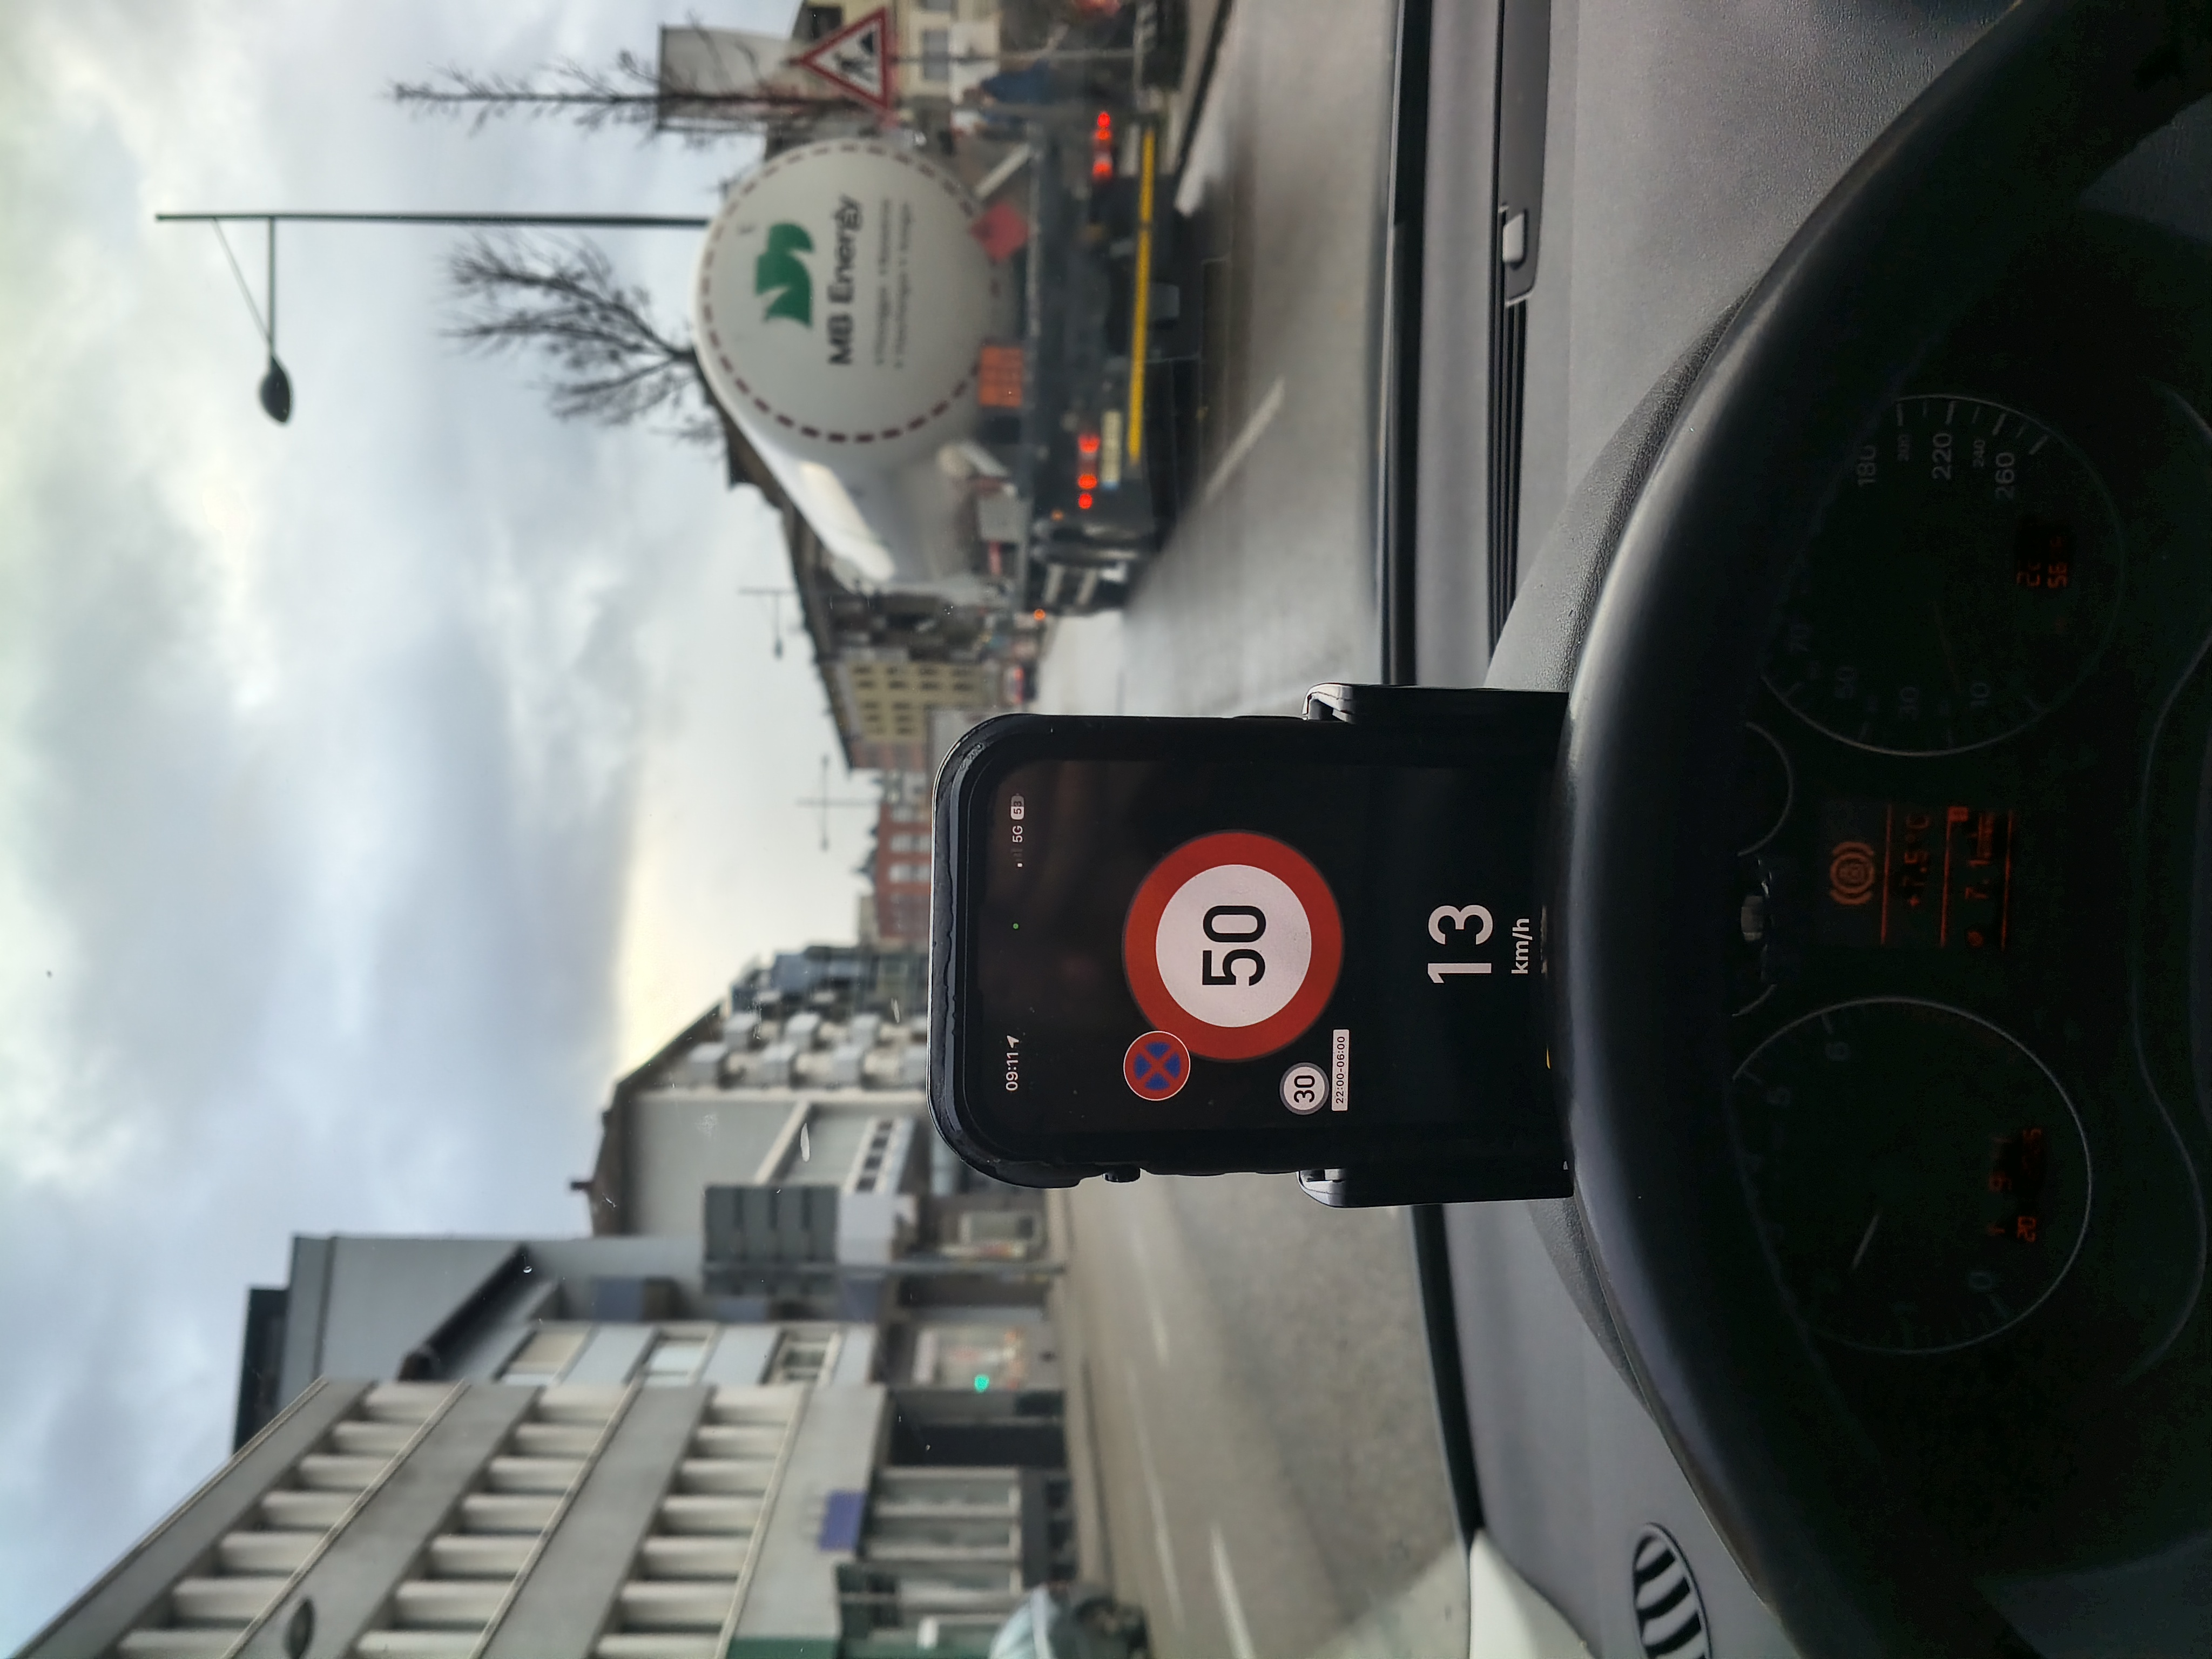
\includegraphics[width=59mm]{v15-youspeed-iphone-limit-portrait-incar.jpg}}
    \end{column}
  \end{columns}
\end{frame}

\begin{frame}{Offene Fragen}
  \begin{itemize}
    \item Wie kann ein Pforzheimer Branding für youspeed.de das Smart-City-Projekt für Bürger erlebbar machen?
    \item Wie lassen sich bestehende Befahrungsbilder und Verkehrszeichenkataster importieren?
    \item Wie baut die Stadt Pforzheim ihr eigenes Kataster auf?
    \item Wie binden wir MobiData BW an? Welche Straßen und Schilder sollen erfasst werden?
  \end{itemize}
\end{frame}

\begin{frame}
  \centering
  % Lossless PNG conversion of HSPF title.webp for pdfLaTeX.
  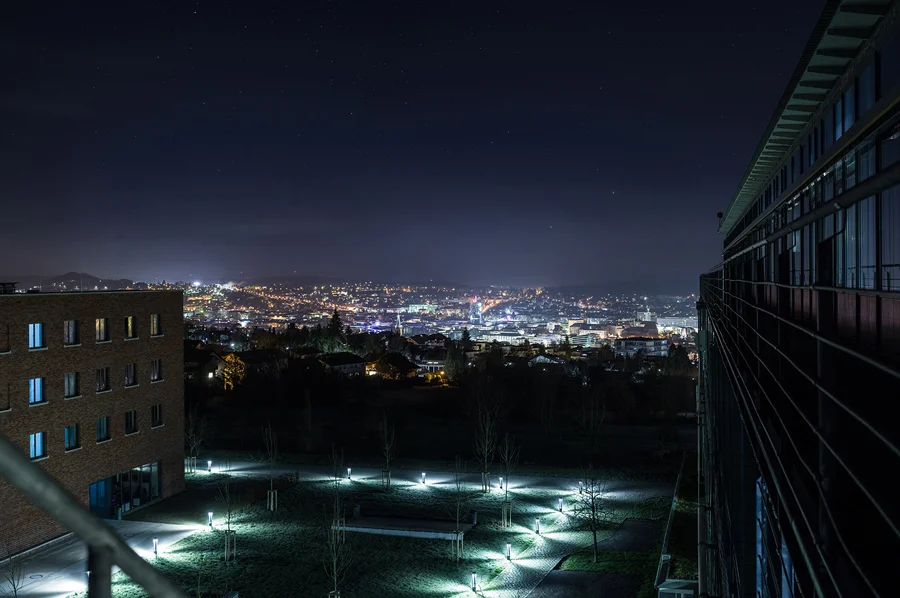
\includegraphics[width=\linewidth,height=74mm,keepaspectratio]{HSPF-title.png}
\end{frame}

\end{document}
